% ------------------------------------------------------------------
\documentclass[12 pt]{article} % A4 paper set by geometry package below
\pagenumbering{arabic}
\setlength{\parindent}{10 mm}
\setlength{\parskip}{12 pt}

% Nimbus Sans font should be reasonably legible
\usepackage{helvet}
\renewcommand{\familydefault}{\sfdefault}
\usepackage[T1]{fontenc}  % Without this \textsterling produces $

% Section header spacing
\usepackage{titlesec}
\titlespacing\section{0pt}{12pt plus 4pt minus 2pt}{0pt plus 2pt minus 2pt}
\titlespacing\subsection{0pt}{12pt plus 4pt minus 2pt}{0pt plus 2pt minus 2pt}
\titlespacing\subsubsection{0pt}{12pt plus 4pt minus 2pt}{0pt plus 2pt minus 2pt}

\usepackage{amsmath}
\usepackage{amssymb}
\usepackage{graphicx}
\usepackage{verbatim}    % For comment
\usepackage[paper=a4paper, marginparwidth=0 cm, marginparsep=0 cm, top=2.5 cm, bottom=2.5 cm, left=3 cm, right=3 cm, includemp]{geometry}
\usepackage[pdftex, pdfstartview={FitH}, pdfnewwindow=true, colorlinks=true, citecolor=blue, filecolor=blue, linkcolor=blue, urlcolor=blue, pdfpagemode=UseNone]{hyperref}

% Put module code and last-modified date in footer
\usepackage{fancyhdr}
\pagestyle{fancy}
\fancyhf{}
\renewcommand{\headrulewidth}{0pt}
\cfoot{{\small \thisunit}\hfill \thepage\hfill {\small \moddate}}

% Hopefully address Canvas complaints about pdf tagging and title
%\usepackage[tagged]{accessibility}
\hypersetup {
  pdfauthor={David Schaich},
  pdftitle={Statistical Physics Computer Project},
}
% ------------------------------------------------------------------



% ------------------------------------------------------------------
% Shortcuts
\newcommand{\Rbb}{\ensuremath{\mathbb R} }
\newcommand{\ubar}{\ensuremath{\overline u} }
\newcommand{\al}{\ensuremath{\alpha} }
\newcommand{\si}{\ensuremath{\sigma} }
\newcommand{\sibar}{\ensuremath{\overline\sigma} }
\renewcommand{\d}[1]{\ensuremath{\mathop{d#1}} }
\newcommand{\vev}[1]{\ensuremath{\left\langle #1 \right\rangle} }
\newcommand{\eq}[1]{Eq.~\ref{#1}}
\newcommand{\showmarks}[1]{\rightline{\texttt{[#1 marks]}}} % \showmarks needs to follow a blank line!
%\newcommand{\TODO}[1]{\textcolor{red}{\textbf{#1}}}
% ------------------------------------------------------------------



% ------------------------------------------------------------------
\begin{document}
\newcommand{\thisunit}{MATH327 Project}
\newcommand{\moddate}{Last modified 4 Feb.~2024}
\begin{center}
  {\Large \textbf{MATH327: Statistical Physics, Spring 2024}} \\[12 pt]
  {\Large \textbf{Computer Project}} \\[24 pt]
\end{center}

\section*{Overview and instructions}
In this computer project you will numerically analyze two types of diffusive behaviour in one-dimensional random walks.
After warm-up exercises on pseudo-random numbers and inverse transform sampling, analyzing ordinary diffusion will allow you to verify your numerical results by comparing them with exact analytic predictions based on the law of large numbers and central limit theorem.
You will then adapt these verified numerical methods to consider \textit{anomalous diffusion}, where exact analytic predictions are not available.

There are five exercises below, four of which provide relevant background information in addition to the tasks for you to complete.
While the exercises mention some syntax specific to Python, you may use a different programming language if you prefer.
\href{https://tinyurl.com/math327demo}{This demo} illustrates all the Python programming tools needed for the project.
For any reasonable programming language, the numerical computations for each exercise should complete in a few minutes or less.

This project is \textbf{due Tuesday, 20 February}.
Submit your work by file upload \href{https://canvas.liverpool.ac.uk/courses/69036/assignments/263364}{on Canvas}.
\textbf{Both} your answers to the questions below and the code that produces your results must be submitted.
These can be uploaded in multiple files or in a tar/zip archive, as you prefer.
With the exception of Mathematica \texttt{.nb} files, it will be quicker for me to check code submitted in its native format (for example, a \texttt{.py} file for Python code or a \texttt{.m} file for MATLAB code).
Anonymous marking is turned on, and I will aim to return feedback by 3 March.

By submitting solutions to this assessment you affirm that you have read and understood the \href{https://www.liverpool.ac.uk/media/livacuk/tqsd/code-of-practice-on-assessment/appendix_L_cop_assess.pdf}{Academic Integrity Policy} detailed in Appendix L of the Code of Practice on Assessment.
Use of resources beyond the module materials (for example, asking ChatGPT to help debug your code) must be explicitly referenced in your submissions.
Clear and neat presentations of your workings and the logic behind them will contribute to your mark.
The marks achieved on this assessment remain provisional until they are ratified by the Board of Examiners in June 2024.
% ------------------------------------------------------------------



% ------------------------------------------------------------------
\newpage % WARNING: FORMATTING BY HAND
\section*{Exercise 1: Pseudo-random numbers}
\subsection*{Background}
We have discussed how statistical physics is based on considering systems that involve some element of randomness.
Because computer programs are deterministic, it is not possible to use them to generate a truly random sequence of numbers.\footnote{New quantum technologies are being developed as a way to produce truly random numbers.  This is part of the motivation for \href{https://uknqt.ukri.org}{large investments in quantum technologies} around the world.}
Instead, computer algorithms generate \textit{pseudo}-random numbers, which are entirely sufficient for our purposes.

A sequence of pseudo-random numbers \textit{appears} random in the sense that knowing the first $N - 1$ elements in the sequence does not suffice to predict the $N$th element with a high probability of correctness.
Equivalently, it takes a very large number of elements for the sequence to start repeating itself.
Such repetition \textit{will} eventually happen, because computers encode numbers in a finite set of bits, which can represent only a finite set of numbers.
For example, $32$ bits can represent all integers from $0$ through \href{https://en.wikipedia.org/wiki/4,294,967,295}{$2^{32} - 1 \sim 10^9$}, while $64$ bits increase the upper bound to $2^{64} - 1 \sim 10^{19}$.
\href{https://docs.python.org/3/library/random.html}{Python uses the Mersenne Twister algorithm} as its default pseudo-random number generator (PRNG).
This algorithm can provide $2^{19937} - 1 \sim 10^{6001}$ numbers before its sequence repeats.

We can view the absence of true randomness as an advantage rather than a limitation.
Deterministic pseudo-random numbers allow our computer programs to be reproducible up to the (very high) precision of the computer.
Each exercise below starts by initializing the PRNG with a ``seed''.
Given the same seed, the PRNG will generate the same sequence of pseudo-random numbers.
In Python, as shown in the demo, this initialization is done by calling the function \texttt{random.seed(s)}, where $s$ is the seed we specify.

\newpage % WARNING: FORMATTING BY HAND
\subsection*{Task}
The Python function \texttt{random.random()} generates a pseudo-random number $u$ with the uniform probability distribution
\begin{equation}
  \label{eq:uniform}
  p(u) = \left\{\begin{array}{l}1 \qquad \mbox{for } 0 \leq u < 1 \\
                                0 \qquad \mbox{otherwise}\end{array}\right. .
\end{equation}
Clearly $\int p(u) \d{u }= \int_0^1 \d{u} = 1$, as required.
What are the exact mean $\mu$ and standard deviation \si of this probability distribution?

\showmarks{2}

Initialize the PRNG with seed $s = 314159$.
For each of the five $R = 20$, $200$, $2000$, $20{,}000$ and $200{,}000$, generate a sequence of $R$ pseudo-random numbers $u_r$ distributed according to $p(u)$.
Don't re-initialize the PRNG when changing $R$, or else these sequences will partially duplicate each other.
Use each sequence to estimate the mean and standard deviation via the law of large numbers,
\begin{align}
  \label{eq:mean}
  \ubar_R & = \frac{1}{R} \sum_{r = 1}^R u_r \qquad &
  \sibar_R & \equiv \sqrt{\left(\frac{1}{R} \sum_{r = 1}^R u_r^2\right) - \ubar_R^2}.
\end{align}
How do your numerical results compare to your exact analytic predictions above?
Four significant figures should suffice for these comparisons.

\showmarks{5}

In class (and on page 15 of the lecture notes) we saw $\displaystyle \vev{\left(\ubar_R - \mu\right)^2} \propto 1 / R$.
Let's test this numerically by repeating the five computations of $\ubar_R$ another $99$ times, ignoring $\sibar_R$ for simplicity.
Together with the results you reported above, this gives a total of $100$ estimates of the random variable $\left(\ubar_R - \mu\right)^2$ for each $R$, which we can use to approximate each expectation value as
\begin{equation}
  \overline{\left(\ubar_R - \mu\right)^2} \equiv \frac{1}{100} \sum_{i = 1}^{100} \left(\ubar_R - \mu\right)_i^2.
\end{equation}

Rather than reporting your results as numerical values, plot $R \times \overline{\left(\ubar_R - \mu\right)^2}$ vs.\ $R$ and see whether the five points appear approximately constant.
If so, is the size of this constant roughly what you would expect?

\textbf{Hints:} Include $0$ on the y-axis of your plot to maintain a sense of scale.
The Matplotlib Python plotting library provides (via its \texttt{pyplot} module) the option \texttt{xscale(`log')} that sets a logarithmic scale for the x-axis, to produce even spacing between these five $R$.

\showmarks{8}
\vfill
% ------------------------------------------------------------------



% ------------------------------------------------------------------
\newpage % WARNING: FORMATTING BY HAND
\section*{Exercise 2: Inverse transform sampling}
\subsection*{Background}
The uniform distribution is a bit boring.
Inverse transform sampling is a technique that allows us to consider more interesting probability distributions, while still generating pseudo-random numbers using the \texttt{random.random()} function.
The idea is illustrated by the sketch below.
\begin{center}
  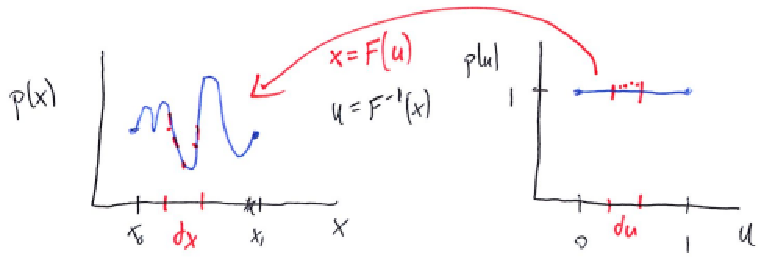
\includegraphics[width=\textwidth]{figs/sampling.pdf}
\end{center}

In words, we take our uniformly distributed $u_r$ and act on them with some invertible transformation $F(u)$ to define $x_r = F(u_r)$ that follow the distribution of interest, $p(x)$.
We require $p(u) \d{u} = p(x) \d{x}$, which allows us to relate $p(x)$ and the inverse transformation $F^{-1}(x)$:
\begin{equation}
  \label{eq:inverse}
  p(x) = p(u) \frac{du}{dx} = p(u) \frac{d}{dx} F^{-1}(x),
\end{equation}
hence the name ``inverse transform sampling''.
This relation lets us either engineer an appropriate transformation $F(u)$ to produce a desired distribution $p(x)$, or determine the distribution that results from a given transformation.

\newpage
\subsection*{Task}
Based on the uniformly distributed pseudo-random numbers $u$ generated by \texttt{random.random()}, define
\begin{equation}
  \label{eq:transform}
  x = F(u) = \arcsin\left(u\right).
\end{equation}

What is the probability distribution $p(x)$ of these random numbers $x$?
What are the minimum and maximum possible values that $x$ can take?
What are the resulting exact mean $\mu$ and standard deviation \si of $p(x)$?

\showmarks{5}

Reset by initializing the random number generator with seed $314159$.
Now, using the \texttt{arcsin} function provided by Numerical Python (NumPy), generate $R = 2{,}000{,}000$ pseudo-random numbers $x_r$ via \eq{eq:transform}.
Use these to numerically estimate the mean and standard deviation of $p(x)$, analogously to \eq{eq:mean} in the previous exercise.
How do your numerical results compare to your exact $\mu$ and \si above?
Four significant figures should suffice for these comparisons.

\showmarks{5}

In a single plot, compare the histogram of the $2{,}000{,}000$ $\left\{x_r\right\}$ to the analytic $p(x)$ you found above.
Do your numerical results match your prediction?
Roughly $51$ bins in the histogram should suffice for this comparison.

\textbf{Hint:} The demo shows how Matplotlib can \texttt{plot} a function $p(x)$ on top of a histogram produced using its \texttt{hist} routine.

\showmarks{5}
% ------------------------------------------------------------------



% ------------------------------------------------------------------
\newpage % WARNING: FORMATTING BY HAND
\section*{Exercise 3: Random walks}
\subsection*{(a) Central limit theorem}
Now consider a random walk that consists of $N$ steps, with the length of each step being a pseudo-random number $x_i$ obtained using \eq{eq:transform}.
By independently generating $R$ different $N$-step random walks you can analyze the final positions of the walks,
\begin{align*}
  X_r(N) & = \sum_{i = 1}^N x_i &
  r & = 1, 2, \cdots, R.
\end{align*}
Based on the central limit theorem in the limit $R \to \infty$, what are the analytic predictions for $\vev{X(N)}$ and the diffusion length
\begin{equation*}
  \ell_2(N) \equiv \sqrt{\vev{\left[X(N)\right]^2} - \vev{X(N)}^2},
\end{equation*}
each as a function of $N$?
[In the lecture notes, $\ell_2(N)$ is called $\Delta X(N)$; the new terminology will be useful for Exercise~5.]

\showmarks{2}

\subsection*{(b) Fixed number of steps}
Reset by initializing the random number generator with seed $314159$.
With fixed $N = 100$, generate $R$ $100$-step random walks for each of $R = 20$, $200$, $2000$, $20{,}000$ and $200{,}000$.
Use the five resulting sets $\left\{X_r\right\}$ to numerically estimate both
\begin{align*}
  \overline{X(N)}_R & \equiv \frac{1}{R} \sum_{r = 1}^R X_r(N) \qquad &
  \overline{\ell_2(N)}_R & \equiv \sqrt{\left(\frac{1}{R} \sum_{r = 1}^R \left[X_r(N)\right]^2\right) - \overline{X(N)}_R^2}.
\end{align*}

How do your numerical results compare to your $R \to \infty$ analytic predictions for $N = 100$?
Five significant figures should suffice for this comparison.

\showmarks{8}

\subsection*{(c) Diffusion constant}
Reset by initializing the random number generator with seed $314159$.
Then fix $R = 20{,}000$ and compute $\overline{\ell_2(N)}_R$ for \textit{every} $N = 1, 2, \cdots, 500$.
Rather than reporting results as numerical values, plot $\overline{\ell_2(N)}_R$ vs.\ $N$.
(\textbf{Hint:} You can ignore potential correlations between $\overline{\ell_2(N)}_R$ for different values of $N$.)

\showmarks{6}

Now fit your numerical results to the function
\begin{equation*}
  \overline{\ell_2(N)}_R = C + D \sqrt{N}.
\end{equation*}
Include your fit in your plot of $\overline{\ell_2(N)}_R$ vs.\ $N$.
How do your fit results for $C$ and $D$ compare to your $R \to \infty$ analytic predictions from the central limit theorem?
(\textbf{Hint:} NumPy's \texttt{polyfit} routine can handle fits linear in $\sqrt{N}$.)

\showmarks{4}
% ------------------------------------------------------------------



% ------------------------------------------------------------------
\newpage % WARNING: FORMATTING BY HAND
\section*{Exercise 4: Cauchy--Lorentz distribution}
\subsection*{Background}
So far we have been able to verify our numerical results by using the central limit theorem.
We now turn to a case in which the central limit theorem will not be applicable, by considering
\begin{align}
  \label{eq:cauchy}
  p_C(x) & = \left(\frac{1}{b \pi}\right) \frac{1}{1 + (x / b)^2} &
  x & \in \Rbb,
\end{align}
which is known as the Cauchy--Lorentz (or just Cauchy) distribution.
Here $b$ is a constant parameter that controls the width of the peak around $x = 0$.
The figure below illustrates this by plotting $p_C(x)$ for each of $b = 1 / 2$, $b = 1$ and $b = 2$, comparing them to the gaussian distribution $\displaystyle \frac{1}{\sqrt{2\pi}} e^{-x^2 / 2}$.

\begin{center}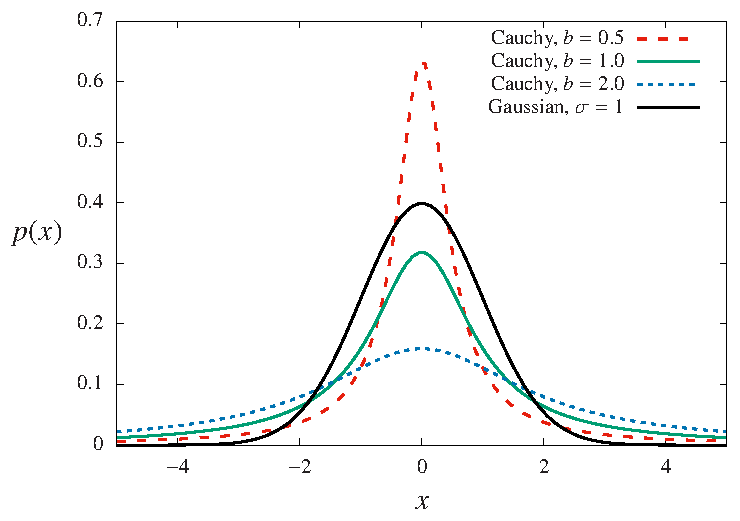
\includegraphics[width=0.75\textwidth]{figs/cauchy.pdf}\end{center}

The figure shows how the peak of the Cauchy--Lorentz distribution around $x = 0$ becomes higher and narrower as $b$ decreases.
Even when its peak is very narrow, as $|x|$ increases $p_C(x)$ again becomes larger than the gaussian distribution, simply because the latter decreases exponentially quickly while $p_C(x)$ decreases only $\sim 1 / x^2$.
These ``fat tails'' at large $|x|$ make the Cauchy--Lorentz distribution both interesting and challenging to analyze.

\newpage % WARNING: FORMATTING BY HAND
\subsection*{Task}
Fix $b = 1$ in the Cauchy--Lorentz distribution, so that \eq{eq:cauchy} becomes
\begin{align}
  \label{eq:px}
  p_C(x) & = \left(\frac{1}{\pi}\right) \frac{1}{1 + x^2} &
  x & \in \Rbb.
\end{align}
Evaluate the integral of this distribution over its full range, $\displaystyle \int_{-\infty}^{\infty} p_C(x) \d{x}$.

\showmarks{2}

Our usual starting point to analyze a probability distribution $p(x)$ is to find its mean and standard deviation, by evaluating
\begin{align*}
  \vev{x} & = \int x \; p(x) \d{x} &
  \vev{x^2} & = \int x^2 \; p(x) \d{x}.
\end{align*}
For the Cauchy--Lorentz distribution in \eq{eq:px}, consider instead the functions
\begin{align*}
  f(a) & = \int_{-a}^a x \; p_C(x) \d{x} = \frac{1}{\pi} \int_{-a}^a \frac{x}{1 + x^2} \d{x} \\
  g(a) & = \int_{-a}^a x^2 \; p_C(x) \d{x} = \frac{1}{\pi} \int_{-a}^a \frac{x^2}{1 + x^2} \d{x}.
\end{align*}
How do $f(a)$ and $g(a)$ behave in the limit $a \to \infty$?

\showmarks{4}

To numerically analyze of the Cauchy--Lorentz distribution, the first step is to determine the transform $F(u)$ that will map the uniformly distributed pseudo-random numbers $u$ (\eq{eq:uniform}) to $x = F(u) \in \Rbb$.
What is the transform $F$ that provides $x = F(u)$ distributed according to $p_C(x)$ in \eq{eq:px}?

\textbf{Hints:} Guided by \eq{eq:inverse}, it will suffice to propose an ansatz for $F(u)$ based on integrating $p_C(x)$, and then follow the steps in Exercise~2 to confirm that this ansatz produces the desired distribution.
You can choose the \href{https://en.wikipedia.org/wiki/Constant_of_integration}{constant of integration} so that $x \to -\infty$ as $u \to 0$ and $x \to \infty$ as $u \to 1$.

\showmarks{6}

Now reset by initializing the random number generator with seed $s = 314159$.
Generate $R = 2{,}000{,}000$ pseudo-random numbers $x_r = F(u_r)$ using the transform you found.
Plot the histogram of these million $\left\{x_r\right\}$ and check whether it agrees with the Cauchy--Lorentz distribution shown above.

\textbf{Hints:} You will need to set an appropriate range for the x-axis of this histogram.
A range $-10 \leq x \leq 10$ with roughly $201$ bins should suffice to show all the interesting features.
In Python this can be done by providing \\
\centerline{\texttt{bins = np.arange(-10.0, 10.0, 20.0/201.0)}}
to the Matplotlib \texttt{hist} function used previously.
In this exercise it is optional to plot $p_C(x)$ itself on top of this histogram.
If you choose to do so, you may need to adjust its normalization (and you should think about why this is needed).

\showmarks{8}
% ------------------------------------------------------------------



% ------------------------------------------------------------------
\newpage % WARNING: FORMATTING BY HAND
\section*{Exercise 5: Anomalous diffusion}
\subsection*{Background}
The ``fat tails'' of the Cauchy--Lorentz distribution mean that $p_C(x)$ provides larger probabilities for \textit{rare events} with large $|x|$ to occur, compared to the gaussian distribution.
This is illustrated in the figures below, each of which shows a thousand-step random walk in two dimensions --- randomly selecting both the size of each step and the direction $0 \leq \phi < 2\pi$ in which to step.
The walk on the left uses step sizes drawn from a gaussian distribution.
Even in two dimensions, random walks of this sort obey the law of diffusion, with a diffusion length growing proportionally to the square root of the number of steps, $\ell_2(N) \propto \sqrt{N}$.

\noindent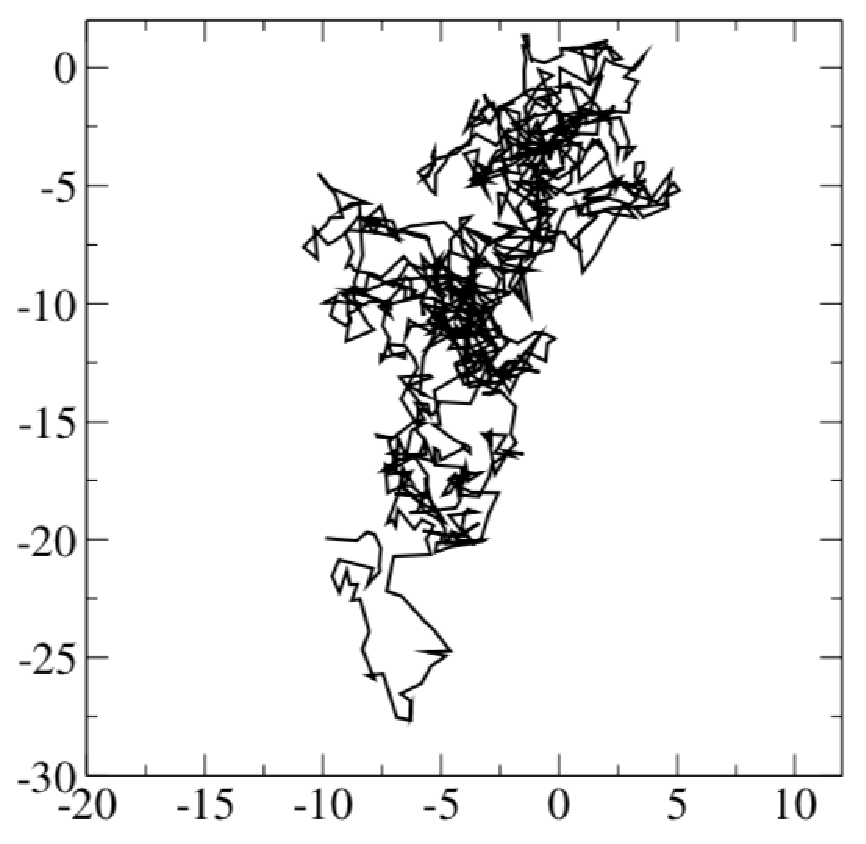
\includegraphics[width=0.45\textwidth]{figs/diffusion_ordinary.pdf}\hfill 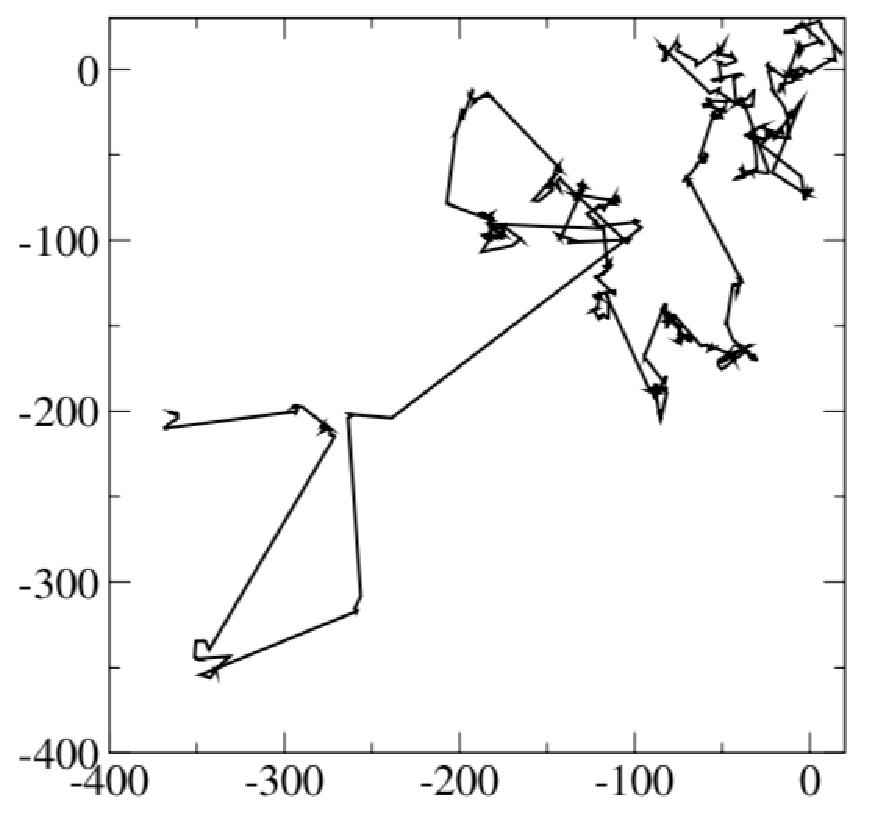
\includegraphics[width=0.45\textwidth]{figs/diffusion_anomalous.pdf}

The walk on the right instead uses step sizes drawn from a Cauchy--Lorentz distribution.
Note that the axes for this figure cover a much larger range!
The fat tails of the Cauchy--Lorentz distribution result in occasional very large jumps, leading to random walks that do not obey the law of diffusion.

Returning to one-dimensional random walks, some of the results from Exercise~4 motivate defining the \textbf{generalized diffusion length}
\begin{equation}
  \label{eq:diff_length}
  \ell_{\theta}(N) = \vev{|X(N)|^{\theta}}^{1 / \theta},
\end{equation}
which depends on a positive real parameter $\theta > 0$.
Since $\theta$ is not necessarily an integer, the absolute value is needed to ensure $\ell_{\theta} \in \Rbb$, rather than becoming complex valued.
If $\vev{X(N)} = 0$ and $\ell_{\theta}$ is well-defined with $\theta = 2$, then this generalized diffusion length could exhibit the ordinary law of diffusion, $\ell_2 \propto N^{1 / 2}$.

For the Cauchy--Lorentz distribution, $\ell_{\theta}$ is ill-defined for any $\theta \geq 1$.
This parameter $\theta$ can take only values $0 < \theta < 1$.
The resulting $\ell_{\theta}$ exhibits \textbf{anomalous diffusion},
\begin{equation*}
  \ell_{\theta}(N) \propto N^{\al},
\end{equation*}
where the exponent is either $\al > \frac{1}{2}$ (called \textit{super-diffusion}) or $0 < \al < \frac{1}{2}$ (called \textit{sub-diffusion}).
This exercise investigates the exponent \al for the distribution $p_C(x)$ in \eq{eq:px}, and explores whether or not \al depends on $\theta$.

\newpage % WARNING: FORMATTING BY HAND
\subsection*{Task a: Fixed number of steps}
Reset by initializing the random number generator with seed $314159$.
With fixed $N = 100$, generate $R$ $100$-step random walks,
\begin{align*}
  X_r(N) & = \sum_{i = 1}^N x_i &
  r & = 1, 2, \cdots, R,
\end{align*}
for each of the four $R = 200$, $2000$, $20{,}000$ and $200{,}000$.
Use the four resulting sets $\left\{X_r\right\}$ to numerically estimate
\begin{equation*}
  \overline{\ell_{\theta}(N)}_R \approx \left[\frac{1}{R} \sum_{r = 1}^R \left|X_r(N)\right|^{\theta}\right]^{1 / \theta}
\end{equation*}
for three values of $\theta = 0.2$, $0.5$ and $0.8$.
(\textbf{Hint:} NumPy provides both an \texttt{abs} function to take the absolute value, and a \texttt{power} function to compute non-integer powers.)

\showmarks{12}

\subsection*{Task b: Anomalous diffusive exponent}
Reset by initializing the random number generator with seed $314159$.
Then fix $R = 20{,}000$ and estimate $\overline{\ell_{\theta}(N)}_R$ for \textit{every} $N = 1, 2, \cdots, 200$, again considering $\theta = 0.2$, $0.5$ and $0.8$.
Instead of reporting your numerical results, plot all three $\overline{\ell_{\theta}(N)}_R$ vs.\ $N$ in a single figure.
(\textbf{Hint:} You can ignore potential correlations between $\overline{\ell_{\theta}(N)}_R$ for different values of $N$.)

\showmarks{8}

Now fit your numerical results for each $\theta = 0.2$, $0.5$ and $0.8$ to the function
\begin{equation*}
  \overline{\ell_{\theta}(N)}_R = D N^{\al}.
\end{equation*}
Report your results for $D$ and $\al$, and comment on their sensitivity to the value of $\theta$.
(\textbf{Hint:} Optionally testing different values of $R$, $N$ or $\theta$ may help to distinguish between real sensitivity vs.\ statistical fluctuations, if you are unsure whether or not an observed effect is significant.)

\showmarks{10}
% ------------------------------------------------------------------



% ------------------------------------------------------------------
\end{document}
% ------------------------------------------------------------------
